\chapter{Introducción} 
\label{chapter:introduccion}
\label{section:introduccion}
\glsresetall

\begin{center}
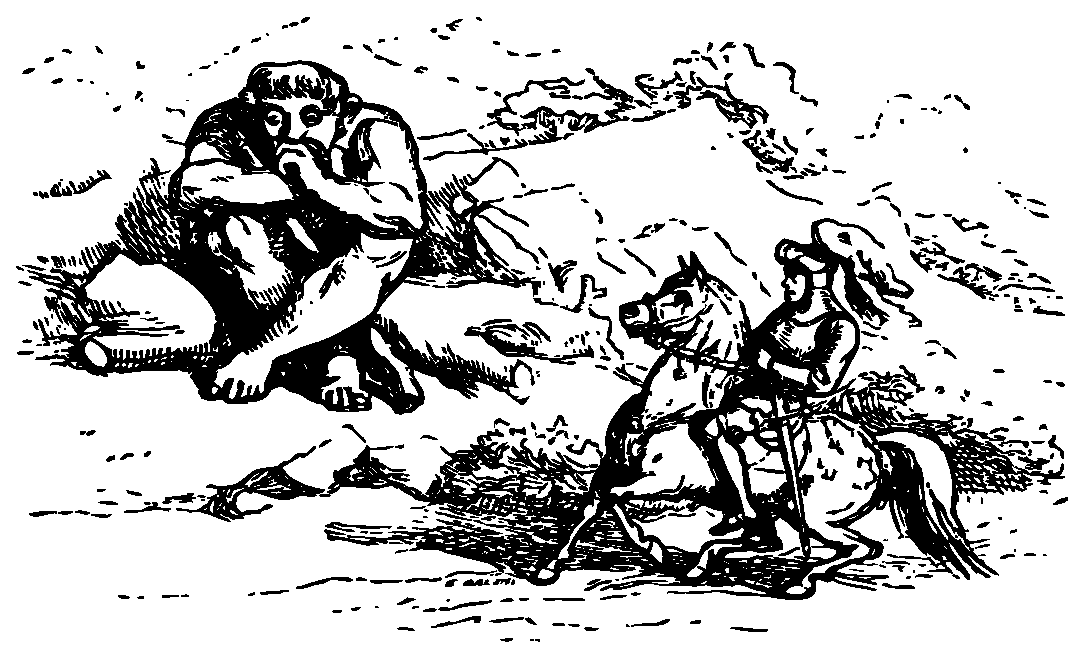
\includegraphics[scale=0.4]{../graphics/johnny_automatic_Jack_and_the_giant.eps}
\end{center}

\lettrine{D}{esde la Revolución Industrial} hasta ahora, la \textit{Era de la Información} \cite{web:informationage}, la humanidad ha cambiado por completo su manera de vivir, de pensar y de actuar. Actualmente la tecnología se ha convertido en un pilar fundamental en el progreso humano. Utilizándola como herramienta hemos sido capaces de salvar vidas, de construir edificios imposibles o incluso de conectar en el momento a personas separadas por miles de kilómetros de distancia. Y no sólo eso, en la actualidad, la manera que tenemos de consumir la información ha cambiado notablemente en los últimos 20 años. Que estamos inmersos en un mundo lleno de datos, de posibilidades, de constantes decisiones\ldots{} no es un hecho, es una realidad.

Se podría decir que el punto de inflexión lo marca la creación de Internet y su posterior expansión al público en general. Hoy en día con un móvil en nuestra mano accedemos a Google \cite{web:google}, consultamos el correo electrónico y estamos en contacto con nuestros seres queridos. Hemos sido testigos de como cada sector de la sociedad ha ido sucumbiendo, en mayor o menor medida, a las \q{maravillas} del progreso tecnológico. Algunos, en cambio, como es el sector educativo todavía se encuentran en fases tempranas de adaptación. Pero, lo que no es discutible es que existen diversos esfuerzos que tratan de crear lo que se podría denominar como \textit{Educación 2.0} \cite{web:educacion20}.

En el mercado actual existen aplicaciones o plataformas que se dedican a la educación a distancia (conocido también como \textit{e-learning} \cite{web:elearning}) para intentar llevar los procesos de enseñanza y aprendizaje a un nuevo nivel. Las ventajas que presentan esta forma de instruir son múltiples ya que eliminan ciertos factores intrínsecos a la educación tradicional como, por ejemplo, las barreras que suponen el espacio o el tiempo. Así mismo añaden mejoras en la forma de asimilar nuevos contenidos puesto que la información fluye de manera asíncrona, es decir, no hace falta tener un diálogo en directo entre la persona que imparte una materia y la que la recibe.

Otros proyectos, como puede ser \alma{} y que es el que tratamos en este escrito, surgen más bien como una necesidad de \textit{complementar} a la educación tradicional sin pretender, de ninguna manera, sustituirla por completo.

Por lo tanto, a lo largo de este proyecto se buscarán las fórmulas adecuadas para poder llevar a cabo con éxito los ideales de \alma{} que no son, ni más ni menos, que facilitar las tareas de gestión y administración utilizando para ello los \profiles{} \cite{web:explicacion-profiles} (que es una herramienta incluida dentro de la plataforma que hemos elegido y adaptado a nuestras necesidades: \tiki{} \cite{web:tikiwiki}).

\section{Objetivos del proyecto}

El objetivo fundamental de este proyecto titulado \q{\work{Gestión dinámica de grupos en una plataforma virtual basada en \tiki{}}} es doble: por una parte trata de \textit{explicar} de manera \textit{clara} y \textit{concisa} el funcionamiento de los \profiles{}. Al finalizar la lectura de este \pfc{} el lector debería ser capaz de poder crear nuevos \profiles{} que le permitan administrar la plataforma \alma{} (o cualquier otra basada en \tiki{}), así como la comprensión del funcionamiento interno de dicha herramienta de automatización. Por otra parte, se desarrollan (y se explican) unos \profiles{} preparados por el autor del escrito que atienden a las necesidades concretas de \alma{}.

En la \figureref{flujo_trabajo} se muestra el flujo de trabajo utilizado en el desarrollo de este \pfc{}:

\begin{figure}[htp]
\centering
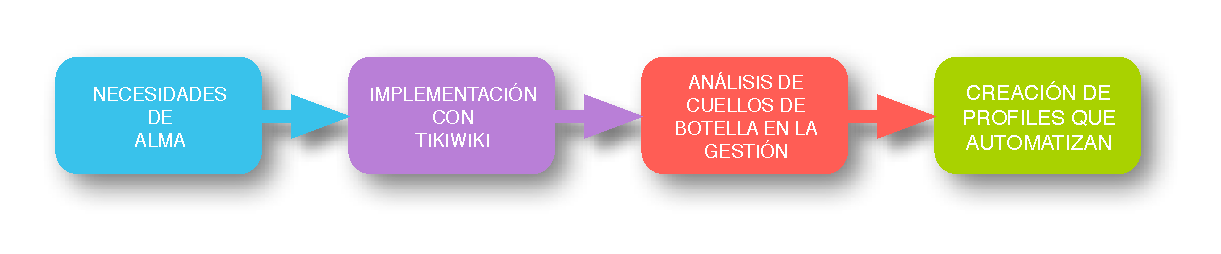
\includegraphics[width=\linewidth]{../graphics/flujo_del_pfc.eps}
\caption{Fases principales del proyecto.}\label{fig:flujo_trabajo}
\end{figure}

\section{Organización del documento}
\label{section:organizacion-documento}

Este \pfc{} está dividido en tres partes:

\begin{enumerate}
\item La primera titulada \work{Entendiendo ALMA y TikiWiki} tratará de explicar de manera detallada qué es el proyecto \alma{}, sus motivaciones, sus implicaciones, los casos de uso\ldots{} (\chapterref{estado-cuestion}), posteriormente se analizarán las diversas opciones para implementar de manera tangible y real el proyecto utilizando herramientas de \textit{software} libre: \tiki{} en nuestro caso (\chapterref{eleccion-software-wiki}).
En el \chapterref{conceptos-fundamentales-tiki} se profundizará con mayor detalle en los conceptos fundamentales de \tiki{} necesarios para entender el funcionamiento de los \profiles{} (se darán explicaciones concretas a características tan importantes como la gestión de grupos y de permisos, administración de recursos y el concepto de perspectivas).

\item La segunda parte titulada \work{Automatización de recursos con \profiles{}} se sumerge en la búsqueda soluciones concretas para atacar diversos problemas que aparecen con la gestión de una gran comunidad de usuarios.
Se explicará qué son y cómo funcionan los \profiles{} (\chapterref{profiles}). Una vez comprendido su funcionamiento interno podremos entender con detalle los \profiles{} que se han desarrollado para la gestión de \alma{} (\chapterref{gestion-dinamica}).
\end{enumerate}

Se concluye el proyecto con la última parte, \work{Sumario}, en el \chapterref{conclusiones} con las lecciones que se han aprendido a lo largo de todo el desarrollo, una autocrítica de las partes del proyecto susceptibles de mejora y se mostrarán unas ideas de lo que podrían ser las futuras líneas de trabajo. Además, al final del libro, se encuentran disponibles una serie de apéndices que sirven como complemento a la información presentada en el resto del documento. 
